% \documentclass{article}
% \usepackage[utf8]{inputenc}
% \usepackage{amsmath}
% \usepackage{natbib}
% \usepackage{graphicx}
% \usepackage{astrojournals} % Necesario para nombres de revistas en luis-ref.bib
% \usepackage[spanish, es-minimal]{babel}
% \bibliographystyle{apj}


% \title{Catalog of stationary bowshock arcs in the Orion Nebula}

% \begin{document}
% \maketitle

% \section{Observaciones y descricción de los datos }

\label{chap:datos}

Para este estudio se usaron observaciones de unos archivos del \textit{Telescopio Espacial Hubble} (\textit{HST}), debido a que este nos brinda unas imágenes con una excelente resolución angular permitiéndonos estudiar de manera efectiva una gran cantidad de objetos estelares, tales como los objetos LL y los arcos de los proplyds en la Nebulosa de Orión, los cuales  presentan fuertes líneas de emisión de \(\ha{}~\lambda6563\) y \(\oiii{}~\lambda5007\). Es así que en las  imágenes tomadas por el \textit{HST} los choques de proa resultan ser muy visibles en el óptico que en cualquier otras líneas de emisión, puesto que en la cáscara chocada domina la emisión de líneas de recombinación tales como \ha{} y para el caso de líneas generadas a patir de la excitación por colisión dominan esencialmente las de \oiii{}.\\ 

 Por tanto en este trabajo se han usado las imágenes de la cámara \textit{Advanced Camera Survey} a bordo del \textit{Telescopio Espacial Hubble} (\textit{HST} por sus siglas en inglés) como parte del Programa GO-9825 con investigador principal \citet{Bally:2006a}, para identificar los objetos LL y trazar la forma de los choques de proa. Esta cámara cuenta con el filtro F658N lo que indica que son imágenes de \ha{} + \nii{}. La importancia de utilizar estas observaciones radica en que estas imágenes tienen una  buena señal a ruido, debido a que manifiestan grandes tiempos de exposición, permitiéndonos analizar óptimamente las fuentes que se desean estudiar. No obstante una de las desventajas de estás observaciones; es que no tienen una cobertura completa de la Nebulosa de Orión, por ejemplo los objetos LL7 y 4285-458 quedan por fuera de estas imágenes. Otra desventaja palpable de las observaciones del ACS-F658N; es que dichas imágenes están contaminadas por las líneas de \(\nii{}~\lambda6584\).\\

 Para solucionar el problema de la falta de cobertura en las imágenes de Bally, se cuentan con unas observaciones de \citet{Robberto:2013a} las cuales también son de la cámara \textit{Advanced Camera Survey} en su canal \textit{Wide field Channel} (ACS-WFC) (las siglas WFC utilizadas para referirse al canal de la cámara ACS no se debe confundir con WFC del WFPC2, puesto que en este caso significa \textit{Wide Field Camera}), pero con la diferencia de que estas hacen parte del programa Treasury, estas imágenes si tienen una cobertura completa de la Nebulosa de Orión y además presentan una alta señal a ruido. Para solucionar el problema de la contaminación por \nii{}, como veremos en este capítulo contamos con unas observaciones de la cámara  \textit{Wide Field and Planetary Camera 2} (WFPC2) también de Robberto. La resolución de las imágenes de esta cámara es muy baja, los pixeles de los detectores son más grandes por un factor de \(\sim2\) en comparación al ACS pero el ``point-spread function'' (PSF) queda igual, entonces no es mostrada adecuadamente en los pixeles del WF del WFPC2 y esto implica un problema a la hora de sustraer la PFS de un objeto del fondo mucho más débil, además la eficiencia del instrumento en comparación al ACS es mucho más baja. Pero alvergan la ventaja de que tiene el filtro F656N que sólo deja pasar las líneas de \ha{} con una contaminación mínima de la línea de \nii{} como se puede ver en la figura~\ref{fig:transmision}. Entonces se usarán estas observaciones para separar las líneas de \ha{} de las líneas de \nii{} en la observaciones de Bally. Puesto que necesitaremos el brillo superficial de \ha{}, para determinar la densidad electrónica y presión térmica en la cáscara chocada de los objetos LL y proplyds.\\

 \begin{figure}
   \centering
    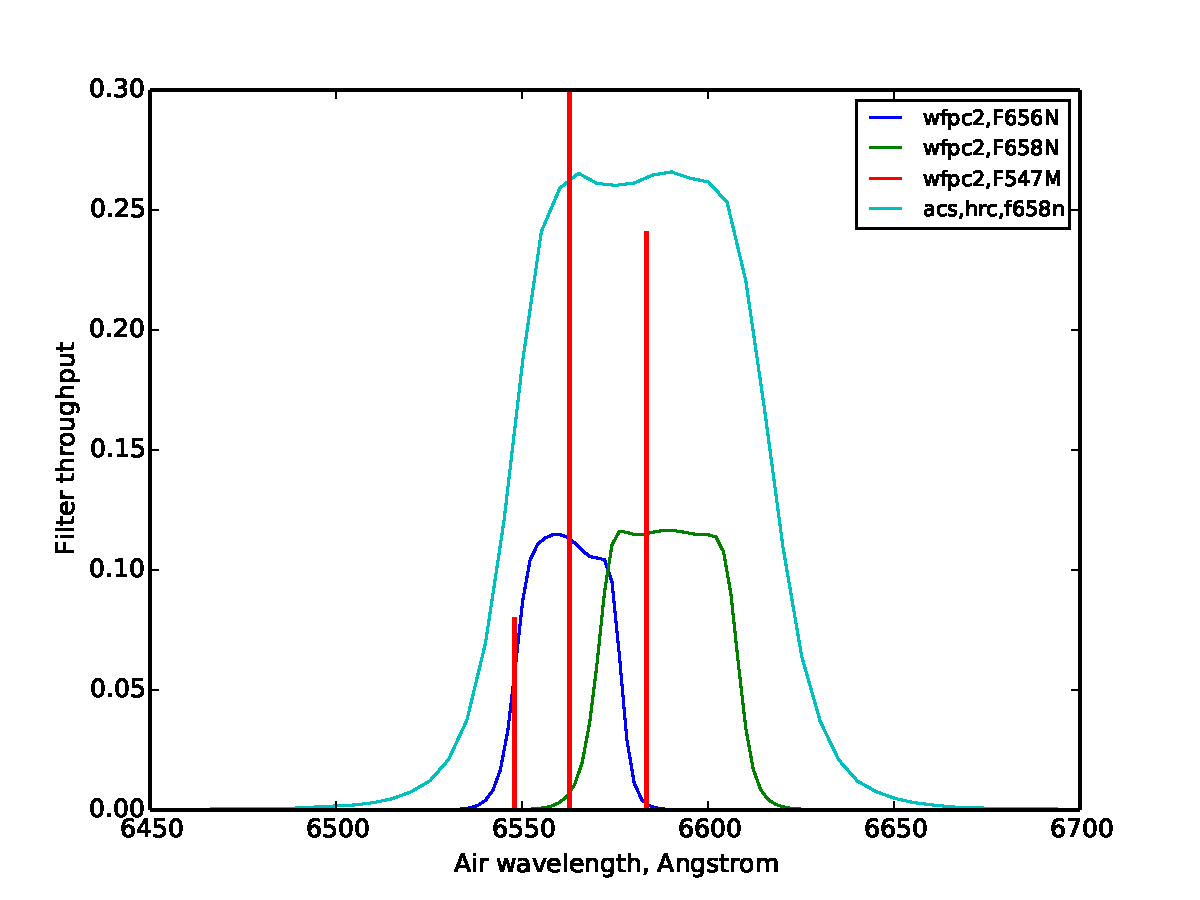
\includegraphics[width=\linewidth, trim=0.7 0.7 0.7 30, clip]{luis-programas/will-filter}
   \caption{Curvas de transmisión de los filtros; F656N y F658N  de la cámara WFPC2 y del filtro F658N de la cámara ACS. Las líneas verticales de color rojo representan en el mismo orden las líneas de emisión de: \nii{} 6548~\A{}, \ha{} 6563~\A{}, \nii{} 6583~\A{}. }
   \label{fig:transmision}
 \end{figure}

Por último, contamos con  las observaciones de unos viejos mosaicos de la cámara WFPC2 como parte del programa GTO-5085. Además de las desventajas de esta cámara mostradas arriba, otra desventaja que tienen estas observaciones es que la cobertura es mas restringida, particularmente las observaciones del PC que solo cubren el centro de la nebulosa con radio menor a medio minuto de arco aproximadamente. Pero estas tienen la ventaja que con la implementación de los filtros f656n y f658n en este programa, se obtuvieron imágenes de \ha{} y \nii{} separadamente, útiles para la verificaión de la calibración del flujo. En este programa se tamaron imágenes del continuo usando el filtro f547m, útil en nuestro caso para hacer la correción del brillo superficial por la contribución del continuo. Finalmente, tenemos un mosaico de unas imágenes de \oiii{}, obtenidas mediante el uso del filtro f502n durante las visitas del \textit{HST}, estas imágenes nos van a permitir ver los objetos de alta ionización en las regiones cercanas del Trapecio donde las estrellas son más débiles comparadas con los arcos vistas con este filtro Otra utilidad de usar estos datos más antiguos es que nos permite distinguir entre los arcos estacionarios y los ecos de objetos HH por su movimiento propio. A continuación daremos una descripción más detallada del juego de observaciones utilizadas en esta tesis.        

\section{La cámara ACS-WFC, El programa GO-9825 y el filtro F658N }
\label{sec:acs}

La cámara ACS-WFC está basada en un masaico de dos detectores CCD de 2048 \(\times\) 4096 pixel. La óptica del instrumento ofrece una escala espacial de aproximadamente 50~\(\mathrm{mas~pixel^{-1}}\), correspondiendo a un campo de visión  de \(202'' \times 200''\). Con esta cámara se cuenta con la presencia del filtro F658N (\ha{} + \nii{}), el cual está destinado al mapeo del material circunestelar de las estrellas con la más alta resolución posible, sobre todo para discriminar fuentes extendidas y evaluar la presencia de emisión circunestelar \citep{Robberto:2013a}.\\

\begin{table}
  \centering
  \small\raggedright
\renewcommand{\arraystretch}{1.5}
  \caption{Observaciones de las cámara ACS y WFPC2}\label{tab:instru}
  \begin{tabular}{l l c c c}
   \hline
   \hline
   Instrumento&      Filtro&      Programa&      Línea de emisión&     Tiempo de exposición (s)\\ \hline
   ACS-WFC&          F658N (Banda ancha)&       GO-9825&       \ha{} + \nii{}&       500\\ 
   ACS-WFC&          F658N (Banda ancha)&        Treasury&   \ha{} + \nii{}&        340\\ 
   WFPC2&            F656N (Banda angosta)&      Treasury&   \ha{}&      400\\
   WFPC2&            f658n&       GTO-5085&      \nii{}&               500\\
   WFPC2&            f656n&       GTO-5085&      \ha{}&                200\\
   WFPC2&            f502n&       GTO-5085&      \oiii{}&              200\\
   WFPC2&            f547m&       GTO-5085&      Continuo&             50\\ 
  \hline
  \end{tabular}
\end{table}
\normalsize

En primer lugar  hemos trabajado con las imágenes de \citet{Bally:2006a}, las cuales son observaciones que han sido obtenidas con la cámara \textit{Wide Field Channel} (WFC) del ACS abordo del \textit{HST}, durante el ciclo 12 del programa GO-9825, donde se obtuvieron 26 imágenes que cubren gran parte de la Nebulosa de Orión, cada imagen fue tomada durante una órbita del \textit{HST}. Las áreas cubierta fueron observadas usando el filtro F658N (\(\ha+\nii\)) y tiempos de exposición de 500 s por punto observado en la nebulosa. Dos posiciones, separadas por \(96''.8\) en el eje-y de los detectores del ACS fueron observados durante cada órbita \citep{Bally:2006a}, correspondiendo a un campo de visión de aproximadamente \(200'' \times 300'' \) para cada imágen resultante \citep{Bally:2006a}. En este sentido las distintas imágenes de la Nebulosa de Orión tomadas durante las 26 órbitas cubrieron un área total de aproximadamente 415 \(\text{arcmin}^{2}\). La figura \ref{fig:fields} muestra la ubicación de cada uno de los 26 campos (visitas) del ACS, donde se han superpuesto en una imagen de \sii{} tomada por el telescopio reflector Mayall ubicado en Kitt Peak cerca de Tucson, para mayor información hechar un vistaso al artículo de \citet{Bally:2001a}. Cada rectángulo representa un campo de cada visita del \textit{HST}.\\

\begin{figure}
  \centering
  \includegraphics[width=.8\linewidth, trim=0.7 0.7 0.7 30, clip]{figuras-tesis/fields-acs-sii.png}
  \caption{Posiciones de los 26 campos del ACS observadas con el \textit{HST} durante el ciclo 12 del programa GO-9825, superpuestas en una imagen de \(\sii\) obtenida con un mosaico de detectores CCD del telescopio reflector Mayall situado en Kitt Peak, Arizona. Los rectágulos representan las imágenes CCD del ACS con un tamaño de \(2046 \times 4096\) pixel cada uno. Esta imagen es tomada de \citet{Bally:2006a}.}
  \label{fig:fields}
\end{figure}

La importancia de utilizar las imágenes de Bally radica en que la señal a ruido es muy buena, debido a que tienen tiempos más largos de exposición, con esto  lograron que el detector CCD recojiera el mayor número de fotones posibles por pixel, implicando que la señal sea muy alta en comparación al ruido. Para nuestro trabajo vamos a utilizar estas imágenes para trazar la forma de los arcos de proa radiativos de las estrellas LL~Ori, puesto que en estas imágenes se logran ver de manera clara los límites de la cáscara chocada.\\

Por otro lado, como ya se dijo arriba esta cámara (ACS) contiene el filtro F658N, el cual es un filtro de banda ancha (\(50 \text{Å}\)), que permite obtener imágenes de \ha{} + \nii{}, donde principalmente domina las líneas de \ha{} y en menor grado las líneas de \nii{}. Sin embargo, la desventaja de utilizar estas observaciones es que no tiene una cobertura completa de la Nebulosa de Orión\footnote{Los objetos, LL7 y 4285-458 quedan por fuera de los campos de Bally.} y además estas observaciones están contaminadas por líneas de \nii{}. Por último es importante señalar que de los 26 campos del ACS-F658N que mapean la región, nuestros objetos se encuentran distribuidos en los campos: 01, 02, 06, 07, 08, 09, 14, 16, 17 y 24. En la figura \ref{fig:field-01} se muestra como es la apariencia de uno de estos campos (visita) de la cámara ACS.\\

\begin{figure}
  \centering
  \includegraphics[width=.95\linewidth, trim=60 90 60 60, clip]{figuras-tesis/field-01-acs.pdf}
  \caption{Campo 01 del WFC-ACS; que corresponde a una imagen de \ha{}+\nii{} observadas con el \textit{HST} durante el ciclo 12 del programa GO-9825, usando el filtro de banda ancha F658N, en ella se puede apreciar el Trapecio y algunos choques de proa en sus cercanías.}
  \label{fig:field-01}
\end{figure}

\section{Programa Treasury del Telescopio Espacial Hubble}
\label{sec:wfpc2}

El Programa Treasury del \textit{HST} descrito en el artículo de \citet{Robberto:2013a}, fue destinado para el estudio de las componentes estelares de la ONC en las longitudes de onda del visible. El programa se basa en un total de 104 órbitas (ciclo 13), cubriendo de este modo las regiones más brillantes de la Gran Nebulosa de Orión en el rango del espectro electromagnético que caen en el óptico, usando filtros de banda ancha para obtener la fotometría más precisa del mayor número posible de objetos de baja masa presecuencia principal. Las cámaras a bordo del \textit{HST} usadas para este fin son; la ACS-WFC, la  cámara  WFPC2 y la Near-Infrared Camera and Multi-Object Spectrograph (NICMOS), las imágnes de esta última cámara no son consideradas para este estudio. \\    

\paragraph{La cámara ACS-WFC y el filtro F658N.}
Con la cámara ACS como parte del Programa Treasury se tomaron imágenes en el óptico (estrictamente hablando de \ha{}) de la Nebulosa de Orión cubriendo un área total de 627~\(\mathrm{arcmin^2}\) (correspondiendo a 904~Mpix aproximadamente) como resultado de las 104 visitas del \textit{HST}, usando el filtro F658N y a diferencia de las observaciones de Bally un tiempo de exposición de 304 s. En la figura~\ref{fig:field-acs-the} se logran ver las posiciones de los campos de la camara ACS del Programa Treasury superpuestos en una imagen de la Nebulosa de Orión. \\

\paragraph{La cámara WFPC2 y el filtro F656N-\ha{}.}
La cámara WFPC2 actualmente remplazada por la Wide Field Camera 3 usó 4 CCDs de $800\times800$ pixel a bordo del \textit{HST}. Tres de esos detectores comprenden la \textit{Wide Field Camera} (WFC) y tomaron imágenes de \(150''\times150''\) con una resolución espacial de 100~\(\mathrm{mas~pixel^{-1}}\) el campo de visión de estas imágenes tienen forma de ``L''. El cuarto detector conocido como la  Cámara Planetaria (PC) tomó imágenenes más pequeñas esto es de \(34''\times34''\) correspondiendo a una escala espacial de 46~\(\mathrm{mas~pixel^{-1}}\) y su campo de visión son campos cuadrados \citep{McMaster:2008}. Un compendio de imágenes de Robberto tomadas con la WFPC2, han de brindar otra oportunidad de estudiar los arcos LL de la Nebulosa de Orión. Puesto que la ya mencionada WFPC2, ha tomado un conjunto de imágenes que cubren en su mayoría a la Nebulosa de Orión a diferencia de las imágenes de Bally que no tienen una cubertura total de la misma. Se han usado 104 órbitas del \textit{HST} para dicho fin, como parte del Programa Treasury \citep{Robberto:2013a}. En la figura \ref{fig:fields-robberto} se pueden apreciar los campos (visitas) del WFPC2, que entre otras cosas cubren un área total de 570.5 \(\text{arcmin}^{2}\). El tiempo de exponsición se puede ver en la tabla~\ref{tab:instru}. \\

\begin{figure}
\centering
  \includegraphics[width=.95\linewidth]{./figuras-tesis/acs-theasury}
\caption{\textit{Izquierda}. Campos de la cámara ACS superpuertos en una imagen de JHK de la Nebulosa de Orión de 2MASS. \textit{Derecha}. Representación de los campos del ACS obtenidas a partir de 104 vistitas del \textit{HST}, como parte del \textit{Programa Treasury}. Mapean una área consirable de la Nebulosa de Orión. Las partes partes mas oscuras son las regiones de solapamiento entre las distintas visitas. También se puede ver el número de identificación de cada campo, para ser referenciado. Imagen tomada de \citet{Robberto:2013a}. }\label{fig:field-acs-the}
\end{figure}

\begin{figure}
  \centering
  \includegraphics[width=.95\linewidth]{figuras-tesis/fields-robberto.jpg}
  \caption{Igual que la figura~\ref{fig:field-acs-the} para los campos de WFPC2.}
  \label{fig:fields-robberto}
\end{figure}

Uno de los filtros usados en este ambicioso programa es el filtro F656N. Este es un filtro de banda angosta de \ha{}, que sólo permite el acceso de estas líneas (\ha{}~\(\lambda = 6563~\text{\AA{}}\)), es así que no permite que pasen las líneas de \nii{} (\(\lambda = 6583~\text{\AA{}}\)). Entonces para este trabajo usamos las observaciones de \citet{Robberto:2013a} (WFPC2) debido a que estas imágenes son sólo de \ha{}. En este orden de ideas, la idea de usar las imágenes de la cámara WFPC2-F656N va a permitir que sea posible separar las emisiones de \ha{} de \nii{} en las imágenes de Bally, subsecuentemente  podremos  utilizar estas imágenes de ACS corregida por \nii{} para determinar parámetros astrofísicos tales como el flujo de momento de los arcos de proa y esto es  porque las observaciones de Bally tienen mejor resolución como se dijo arriba.

\section{Otras observaciones de la cámara WFPC2:  viejos mosaicos}
\label{sec:mosaic}

Para este estudio también se cuenta con unas observaciones, un poco más viejas que mapean una región particular de la Nebulosa de Orión (el centro de la nebulosa). Estas observaciones son el resultado de dos pragramas del \textit{HST}, el primero de estos es el programa GTO-5085 (Guaranteed Time Observer  por su nombre en inglés) cuyo principales investigadores fueron  \citet{Odell:1996} y el segundo corresponde al programa GO-5469 (General Observer por su nombre en inglés) con Jhon Bally como principal investigador. Las imágenes proporcionadas por el programa de Bally fueron usadas principalmente para el estudio de proplyds con una  alta resolución espacial, usando la cámara WFPC2 abordo del \textit{HST}. En estas imágenes el tamaño de lo pixeles es de \(0.0996''\) algo muy característico de las cámaras WF \citep{Holtzman:1995}. Los campos seleccionados para la formación de las imágenes se determinaron de tal manera que tengan una cobertura continua de un área en la parte central de la Nebulosa de Orión, en este sentido se tiene una superposición de los campos, representados através de unos  masaicos de la cámara WFPC2. Se hablan de varios mosaicos puesto que se utilizaron múltiples filtros del programa GTO-5085 para registrar diferentes líneas de emisión. Los extremos de la región mapeada fueron elegidos con el propósito de incluir objetos de particular interés, tales como objetos Herbig-Haro en el norte y los choques de proa en el suroeste \citep{Odell:1996}.\\

 Los filtro usados fueron seleccionados de tal manera que se capturaran las líneas de emisión más fuertes, es decir aquellas que representaran un rango razonable de condiciones de ionización. Por tanto se cuenta con un masaico en el que se usó el filtro f658n, es decir en este mosaico domina sólo la presencia de la línea de emisión \nii{} (6584~\A{}). También se cuenta con un mosaico, en el que sólo dominan las líneas de emisión de \ha{} (6563~\A{}), puesto que para capturar las imágenes se usó el filtro f656n. En esta lista se incluye un masaico cuyas imágenes son el resultado del uso del filtro f502n, donde se han registrado las líneas de emisión de \oiii{} (5007~\A{}), que provienen de regiones con la más alta ionización en la nebulosa. Por último existe un mosaico formado por los campos obtenidos a partir del filtro f547m \citep{Burrows:1995}, este es un filtro suficientemente ancho (en comparación a los demás filtros), ubicado en una región del espectro electromagnético, donde no hay líneas fuertes de emisión, por tanto este mosaico son unas imágenes del continuo. Los tiempos de exposición para cada filtro son: f656n;  200~s, f658n; 500~s, f502n; 200~s, f547m; 50~s para el programa GO-5085. 



% \bibliography{luis-ref}

% \end{document}
